\section{Predstavitev podatkov vzorca}

Naredimo preskok iz teorije v prakso. Imamo dva vzorca podatkov in želimo izračunati divergenco med njima. Pojavi se problem, saj ne vemo, kateri porazdelitvi ustrezata dana vzorca, torej nimamo teoretičnih gostot vertjetnosti. Poiskati želimo približek za gostoto verjetnosti. To naredimo z vpeljavo histogramov ali z vpeljavo različnih ocenjevalcev za gostoto verjetnosti.

\subsection{Histogram}\label{pog-histogram}

Naj bo $S$ množica podakov. Razdelimo interval $[\min(S), \max(S)]$ na $n \in \mathbb{N}$ intervalov z dolžino večjo od 0:
\[
[\min(S), \max(S)] = [a_0, a_1) \cup [a_1, a_2) \cup \ldots \cup [a_{n-2}, a_{n-1}) \cup [a_{n-1}, a_n].
\]
Omenimo, da $\min(S) = a_0$ in $\max(S) = a_n$. Naj bo
\[
    N: \{ 0, \ldots, n-1 \} \rightarrow \mathbb{N}
\]
funkcija s predpisom:
\[
N(i) = \sum_{x \in S} \delta_i(x),
\]
kjer je
\[
    \delta_i(x) =
    \begin{cases}
        1, \quad x \in [a_i, a_{i+1}) \\
        0, \quad \text{sicer}
    \end{cases}.    
\]
Če je $i = n - 1$, je v pogoju pri $\delta_{n-1}$ interval zaprt. Funkcija $N$ torej prešteje, koliko elementov iz $S$ je znotraj intervala $[a_i, a_{i+1})$.
\pagebreak
\begin{definicija}
    \textbf{Histogram} je funkcija $H: \mathbb{R} \rightarrow \mathbb{N}$ s predpisom:
    \begin{equation}
        H(x) =
        \begin{cases}
            \ N(i)&, \quad \exists i \in \{ 0, \ldots, n-1\} \ni: x \in [a_i, a_{i+1}) \\
            \quad 0&, \quad sicer 
        \end{cases},
    \end{equation}
    kjer v pogoju pri $i=n-1$ dopuščamo zaprti interval.
\end{definicija}

Pri obdelavi podatkov je bolj kot zgornja različica histograma uporabna naslednja:

\begin{definicija}
    \textbf{Normalizirani histogram} množice podatkov $S$ je funkcija $h: \mathbb{R} \rightarrow \mathbb{R}_+$ s predpisom:
    \begin{equation}
        h(x) =
        \begin{cases}
            \frac{N(i)}{|S|\cdot (a_{i+1} - a_i)}&, \quad \exists i \in \{ 0, \ldots, n-1\} \ni: x \in [a_i, a_{i+1}) \\
            \quad\quad 0&, \quad sicer 
        \end{cases},
    \end{equation}
    kjer v pogoju pri $i=n-1$ dopuščamo zaprti interval.
\end{definicija}

\begin{opomba}
    Normalizirani histogram ima lastnost: $\int_\mathbb{R} h(x) dx = 1$.
\end{opomba}

Poglejmo si zgled histograma in razliko med histogramom in normaliziranim histogramom.

\pagebreak
\begin{zgled}
    $S_0 = \{1,1.3,1,2.5,3,3.5,3.6,4,4.1,4.2,5\}$. \\
    $[\min(S_0), \max(S_0)]$ razdelimo na 4 podintervale: $[1,2), [2,3), [3,4), [4,5]$.
    Poglejmo, kako izgledata histogram in normaliziran histogram (slika \ref{hist-zgled}).
    \begin{figure}[!h]
        \begin{subfigure}{0.49\textwidth}
            \centering
            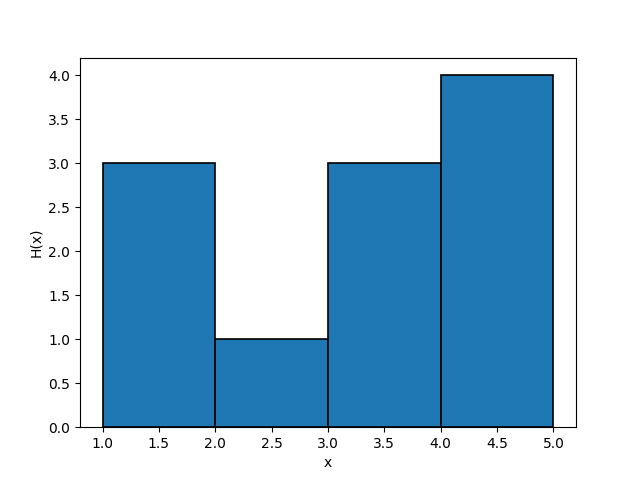
\includegraphics[scale=0.47]{histogram-zgled.png}
        \end{subfigure}
        \begin{subfigure}{0.49\textwidth}
            \centering
            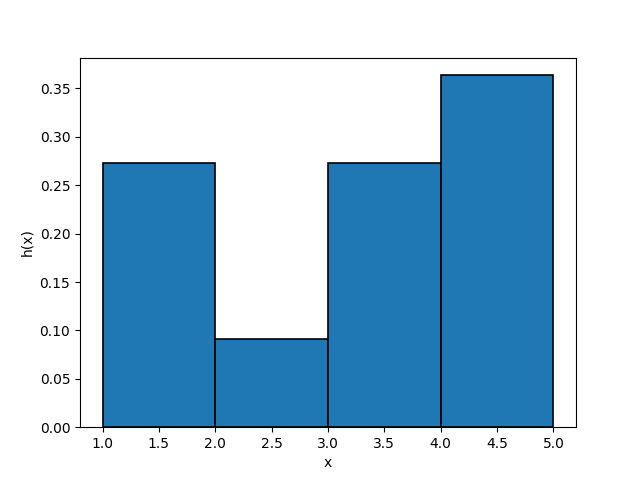
\includegraphics[scale=0.47]{histogram-norm-zgled.png}
        \end{subfigure}
        \caption{Na levi je (navaden) histogram, na desni pa normaliziran histogram vzorca $S_0$. Oblika je ista, razlika je v skali na y-osi.}
        \label{hist-zgled}
    \end{figure}
\end{zgled}

Od zdaj naprej bomo enačili pojma histogram in normaliziran histogram, z obema pa bomo v mislih imeli normaliziran histogram.

V zgledu opazimo, da histogram grafično ni podan kot funkcija. Opišimo  grafičen prikaz histogramov.

\pagebreak
\subsection{Grafični prikaz histogramov}

Histogram je odsekoma konstantna funkcija, kar je razvidno iz definicije ($h(x)$ je konstantna na vsakem intervalu $[a_i, a_{i+1})$). Zato si histogram lahko predstavljamo kot množico pravokotnikov, ki jim pravimo \textbf{stolpci} (angl. bins) histograma.

Naj bo na intervalu $[a_{i}, a_{i+1}), i \in \{0,\ldots,n-1\}$ i-ti stolpec oziroma stolpec i histograma, torej ima histogram $n$ stolpcev. Stolpec i ima širino $w_i = a_{i+1} - a_{i}$. Če so intervali enako dolgi, imajo vsi stolpci isto širino $w$. To širino lahko tudi izračunamo:
\begin{equation}\label{sirina_stevilo}
    w = \frac{\max(S)-min(S)}{n} = \frac{a_n - a_0}{n},
\end{equation}
kjer je n število stolpcev histograma.

Višina i-tega stolpca $h_i$ pa je vrednost funkcije $h$ v poljubni točki znotraj intervala \\ $[a_{i}, a_{i+1})$, torej:
\begin{equation}
    h_i = h(x) \quad \text{za} \quad \forall  x \in [a_{i}, a_{i+1}].
\end{equation}

Zgornji način predstavitve histograma ni uporaben le grafično, temveč tudi računsko. Namesto integrala funkcije $h$ lahko izračunamo vsoto ploščin stolpcev, da dokažemo, da je ploščina histograma enaka 1. Numerično se nam bo to izplačalo, saj je numerično integriranje bolj zahtevno kot računanje osnovnih operacij. Enako velja za izračun divergence, kjer uporabimo integracijo.
\pagebreak
\subsection{Optimalno število stolpcev histograma}

Recimo, da ima množica $S$ porazdelitev $P$. Naj bo $p$ gostota verjetnosti te porazdelitve, $h_n$ pa histogram množice $S$ z $n$ stolpci. Velja:
\begin{equation}
    \lim_{\begin{smallmatrix} |S| \to \infty \\ n \to \infty \end{smallmatrix}} h_n(x) = p(x) \quad \text{za} \quad \forall x \in S.
\end{equation}
Histogram je torej lahko ocena gostote verjetnosti množice $S$.

V nobenem vzorcu nimamo na voljo $\infty$ podatkov, zato moramo paziti na izbiro števila stolpcev histograma. Če je $n>|S|$, bo najmanj en stolpec prazen (oz. bo imel višino 0), torej bo to lahko zelo slab približek za gostoto verjetnosti (npr. normalna porazdelitev je povsod večja od 0). Druga skrajnost je, ko izberemo premalo stolpcev in tako izgubimo podatke o porazdelitvi (moduse, če jih ima vzorec več).


\begin{zgled}
Vzemimo množico $S_0 = \{1,1.3,1,2.5,3,3.5,3.6,4,4.1,4.2,5\}$. Poglejmo si histograme ob različni izbiri števila stolpcev.
\begin{figure}[!h]
    \centering
    \begin{subfigure}{0.3\textwidth}
        \centering
        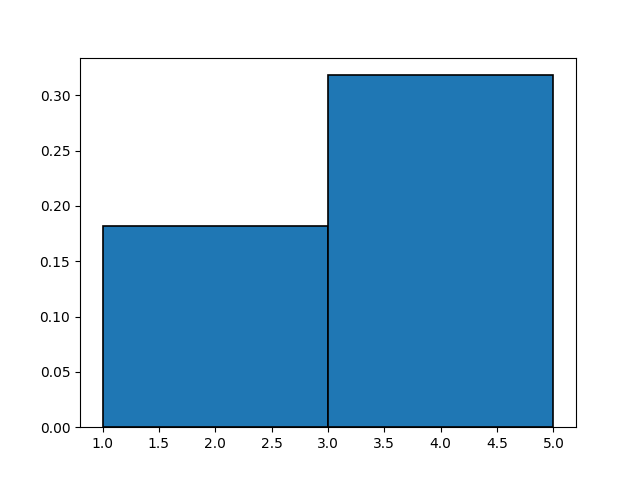
\includegraphics[scale=0.29]{hist-2bina.png}
        \caption{$n=2$}
        \label{2-bina}
    \end{subfigure}
    \begin{subfigure}{0.3\textwidth}
        \centering
        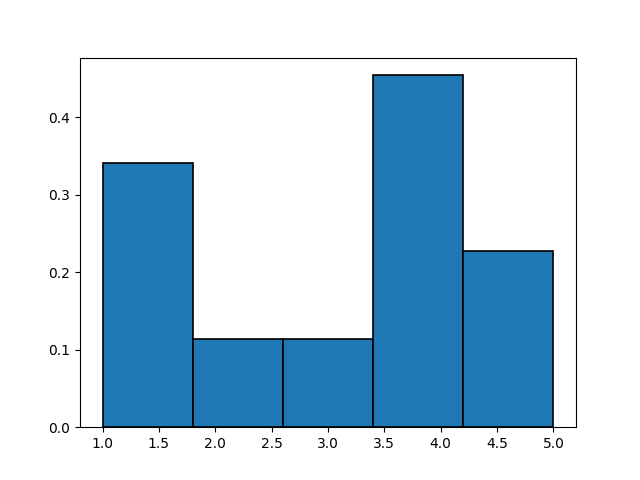
\includegraphics[scale=0.29]{hist-5binov.png}
        \caption{$n=5$}
        \label{5-binov}
    \end{subfigure}
    \begin{subfigure}{0.3\textwidth}
        \centering
        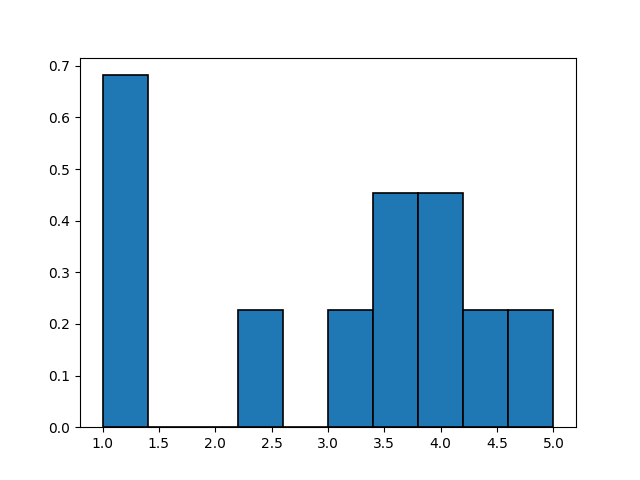
\includegraphics[scale=0.29]{hist-10binov.png}
        \caption{$n=10$}
        \label{10-binov}
    \end{subfigure}
    \caption{Histogrami z različnimi števili stolpcev.}
\end{figure}

V primeru \ref{2-bina} smo izbrali premalo stolpcev, s čimer lahko zgrešimo pomembne lastnosti množice $S$. V primeru \ref{10-binov} pa smo izbrali preveč stolpcev, s čimer dobimo prazne stolpce.
\end{zgled}

Obstaja veliko izbir za optimalno število stolpcev. Naštejmo jih. Za vse izbire naj bo $S$ vzorec in $m = |S|$ moč vzorca.

\pagebreak

\subsubsection{Korenska izbira}
Pri tej izbiri optimalno število stolpcev histograma izračunamo po naslednji formuli:
\begin{equation}
    n = \big\lceil \sqrt{m}\  \big\rceil.
\end{equation}
Izračunamo torej kvadratni koren od števila podatkov v vzorcu in zaokrožimo to število na najmanjše celo število, ki je večje od dobljenega korena.

% preveri alternativo za sklanjanje za Rice.
% PRAVILNO: Riceovo - mi ni všeč
% Kaj, ce je Rice bila zenska? Zaenkrat se izognem sklanjanju
% \subsubsection{Riceovo pravilo}
\subsubsection{Rice}
Pri tej izbiri optimalno število stolpcev za histogram izračunamo na naslednji način:
\begin{equation}
    n = \big\lceil \sqrt[3]{m}\  \big\rceil.
\end{equation}

\subsubsection{Sturges}
Pri tej izbiri optimalno število stolpcev izračunamo po naslednji formuli:
\begin{equation}
    n = \big\lceil \log_2{m}\  \big\rceil + 1.
\end{equation}
Ta formula je zelo varčna, saj logaritem narašča zelo počasi. Medtem ko bo pri korenski izbiri in 10000 podatkov optimalno število stolpcev 100, bo pri Sturgesovi formuli število stolpcev enako 11.

Vse tri do zdaj naštete izbire delujejo zelo naivno, saj upoštevajo le velikost vzorca, ne pa ostalih njegovih lastnosti, npr. variance. Kljub temu pa se izkaže, da te metode zelo dobro konkurirajo z ostalimi, če gledamo lepe porazdelitve, npr. normalne porazdelitve. Težava so bolj kompleksne porazdelitve, ki imajo visoke repe in so na eni strani omejene. Pri teh hitro dobimo premalo stolpcev in moramo nujno upoštevati še kakšno drugo lastnost, ne le velikosti vzorca.

\pagebreak
Poglejmo si sedaj še izbiri, ki upoštevata bolj specifične lastnosti vzorca. Ti dve formuli sicer vrneta optimalno širino stolpca, a zlahka iz tega podatka dobimo optimalno število stolpcev (glej formulo \eqref{sirina_stevilo}). 

\subsubsection{Scoot}
Formula Scoot poleg velikosti vzorca upošteva še njegov standardni odklon $\sigma$:
\begin{equation}
    h = 3,49 \cdot \sigma \cdot m^{-1/3}.
\end{equation}

\subsubsection{Freedman-Diaconis}
Ta izbira prav tako uporabi še dodatno lastnost poleg velikosti vzorca, in sicer medkvartilno razdaljo vzorca $IQR$ (angl. \textit{interquartile range}), to je razlika med zgornjim in spodnjim kvartilom. 
\begin{equation}
    h = 2 \cdot IQR \cdot m^{-1/3}.
\end{equation}

Ker smo že sproti opisali izbire, primer izpustimo. Omenimo pa, da sta zadnji dve metodi v splošnem najboljši, saj poleg velikosti vzorca upoštevata še dodatne lastnosti vzorca, poleg tega pa je izračun variance in medkvartilne razdalje hiter, zato metodi nista časovno potratni.
\pagebreak
\subsection{Enakovredni stolpci}

Do sedaj smo obravnavali samo stolpce, ki so imeli enako širino. Kaj pa, če je mogoče optimalna izbira taka, da stolpci niso enako široki? Eden od takih načinov je vpeljava enakovrednih stolpcev.

\begin{definicija}
    Naj bo $S$ množica podatkov. Naj bo $h$ histogram z $n$ stolpci, $n < |S|$, zgrajen glede na podatke iz $S$. Histogram ima \textbf{enakovredne stolpce}, če je v vseh stolpcih "približno enako" število podatkov.
\end{definicija}

\begin{figure}[!h]
    \centering
    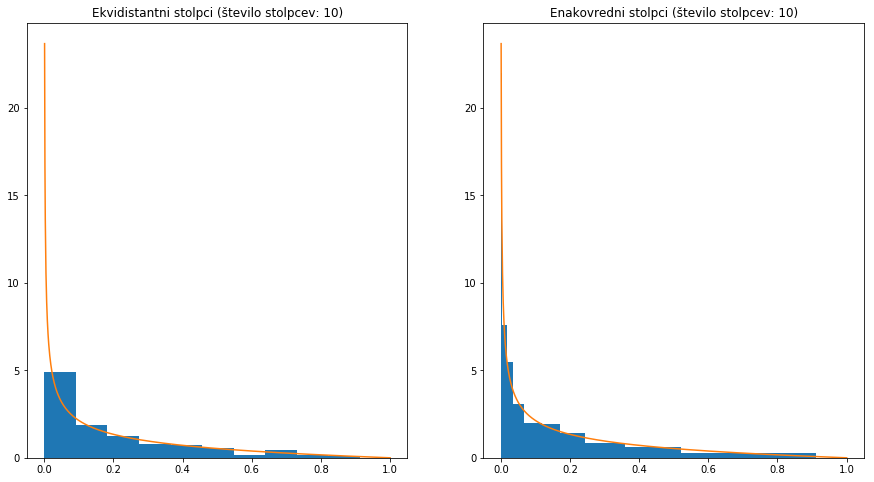
\includegraphics[width=\textwidth]{ekvikvan.png}
    \caption{Primerjava med histogramom z enako širokimi stolpci in histogramom z enakovrednimi stolpci za beta porazdelitev ($\alpha = 0.5$, $\beta = 2$). Vidimo, da se ob istem številu stolpcev veliko bolj prilegajo enakovredni stolpci}
\end{figure}

V zgornji definiciji smo uporabili besedno zvezo "približno enako", ker ni nujno, da je število $|S|$ deljivo s številom $n$. Pri konstrukciji takega histograma pa se temu problemu lahko izognemo recimo tako, da v zadnji stolpec damo toliko podatkov, kolikor je ostanek pri deljenju števila $|S|$ z $n$. Najprej opišimo, kako konstruiramo takšen histogram, nato pa si bomo to pogledali na zgledu.

\subsubsection*{Konstrukcija histograma z enakovrednimi stolpci}

Naj bo $S = \{x_1, x_2, \ldots, x_m\}$ množica podatkov. Konstruirati želimo histogram z $n$ stolpci. Ta histogram bo imel enakovredne stolpce, če bo v vsakem stolpcu $\lfloor m/n \rfloor$ podatkov (razen v zadnjem stolpcu, če število $m$ ni deljivo z $n$ - v tem primeru bomo dobili $n+1$ stolpcev). Potrebujemo meje stolpcev histograma. Enkrat, ko bomo imeli meje, bomo lahko zlahka dobili tudi višine.

Recimo, da je $S$ naraščajoče urejena, sicer pa jo tako uredimo. Naj bo $X$ prazen seznam, v katerega bomo vstavljali meje stolpcev. Prva meja je očitna: $S(1)$, ki je tudi minimalna vrednost množice $S$. Vstavimo torej $S(1)$ v seznam X.

Naj bo $k = \lfloor m/n \rfloor$. v 1. koraku naj bo $S_1$ kopija urejene množice brez prvih $k$ elementov. Nato v seznam $X$ dodamo najmanjši element nove množice $S_1$. Tako bosta v množici $X$ elementa $S(1)$ in $S_1(1)$. V tem stolpcu bo torej ravno $k$ elementov (element $S_1(1)$ bo ležal v naslednjem stolpcu).

Postopek ponavljamo, dokler ni v kopiji množice $S$ manj kot $k$ elementov. Tedaj v seznam $X$ dodamo zadnji, največji element množice $S$.

Višine dobimo tako, da preštejemo število podatkov v posameznem stolpcu, in to število deljimo z $m\cdot w$, kjer je $w$ širina stolpca.

\begin{zgled}
    Vzemimo $S = \{-17, -13, -9, -8, -6, -5.5, 0, 5.5, 6, 9, 10, 10.5, 11, 12\}$, $|S| = 14$. Želimo dobiti 4 enakovredne stolpce. Na začetku je v $X$ najmanjši element $S$, torej $X = [-17]$. Naš $k$ bo enak $\lfloor 14/4\rfloor = 3$. Nadaljujemo po korakih:
    \begin{enumerate}
        \item Iz $S$ odstranimo prve 3 elemente: $S_1 = \{-8, -6, -5.5, 0, 5.5, 6, 9, 10, 10.5, 11, 12\}$. Najmanjšega iz $S_1$ damo v $X$: $X = [-17, -8]$.
        \item IZ $S_1$ odstranimo prve 3 elemente: $S_2 = \{0, 5.5, 6, 9, 10, 10.5, 11, 12\}$. V $X$ dodamo najmanjšega: $X = [-17,-8,0]$.
        \item $S_3 = \{9, 10, 10.5, 11, 12\}$, $X = [-17,-8,0,9]$.
        \item $S_4 = \{11, 12\}$, $X = [-17,-8,0,9,11]$.
        \item V $S_4$ imamo samo dva elementa, zato v $X$ dodamo največjega: $X = [-17,-8,0,9,11,12]$
    \end{enumerate}
    Dobimo torej meje stolpcev $X=[-17,-8,0,9,11,12]$. Višine dobimo tako, da v vsakem stolpcu preštejemo število podatkov in to število deljimo z $14\cdot w$, kjer je $w$ širina stolpca.

    \begin{figure}[!h]
        \centering
        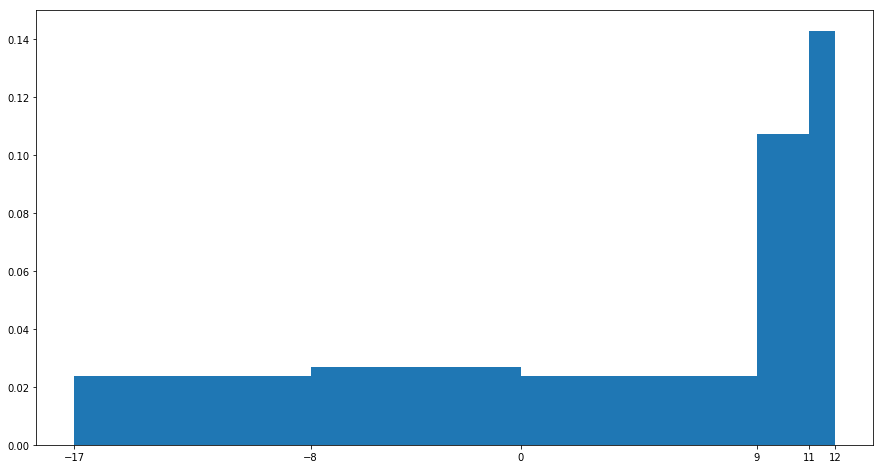
\includegraphics[width=\textwidth]{eqBinsZgled.png}
        \caption{Histogram množice $S$ z enakovrednimi stolpci. Zadnji stolpec vsebuje le 2 podatka, ostali pa 3.}
    \end{figure}

\end{zgled}
\pagebreak
\subsection{Ocena gostote verjetnosti z jedrom}
Opišimo še nekoliko drugačen pristop za predstavitev podatkov. Najprej pa moramo povedati, kaj sploh mislimo z besedo "jedro".
\begin{definicija}
    \textbf{Jedro} je nenegativna realna integrabilna funkcija $K$ z lastnostima:
    \begin{itemize}
        \item $\int_{-\infty}^\infty K(x) \  dx = 1 \quad$ in
		\item $K(-x) = K(x), \quad \forall x \in \mathbb{R} \quad$ (simetrija).
    \end{itemize}
\end{definicija}

\begin{figure}[!h]
    \centering
    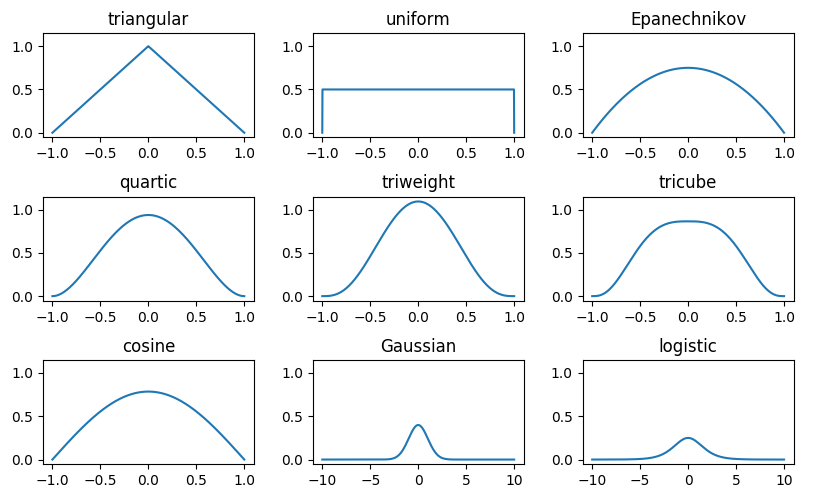
\includegraphics[width=\textwidth]{jedra.png}
    \caption{Nekaj primerov jeder.}
    \label{jedra}
\end{figure}

Ideja ocenjevanja gostote verjetnosti z jedri (angl. \textit{kernel density estimation}) je, da na vsako točko v vzorcu obesimo jedro, ki ga vnaprej določimo, nato pa ta jedra seštejemo in rezultat normiramo. Ker so jedra nenegativna, bo torej pridobljena funkcija ustrezala definiciji gostote verjetnosti.
\begin{definicija}
    \textbf{Ocena gostote verjetnosti z jedrom} je neparametričen način ocenjevanja gostote verjetnosti. Naj bo $K$ jedro in $X = \{x_1,\ldots,x_n\}$ množica podatkov.  Ocena gostote verjetnosti z jedrom $K$ množice $X$ je funkcija, definirana kot:
    \begin{equation}
        f_h(x) = \frac{1}{n\cdot h} \  \sum_{i=1}^n K\Big(\frac{x - x_i}{h}\Big),
    \end{equation}
    kjer je $h$ parameter glajenja, imenovan "bandwidth". % bandwidth == pasovna širina?? mislim da ne
\end{definicija}

Parameter $h$ močno vpliva na končno oceno. Če je $h$ premajhen, lahko dobimo močno oscilirajočo funkcijo, ob preveliki izbiri $h$ pa lahko izgubimo pomembne podatke o porazdelitvi. Če potegnemo vzporednico s podpoglavjem o histogramih, lahko rečemo, da $h$ igra podobno vlogo kot izbira optimalnega števila stolpcev pri histogramih. V optimizacijo paramtra $h$ se ne bomo poglabljali, ponavadi pa ga izračunamo kot:
\begin{equation}
    h = \sigma(X) \cdot \Big(\frac{4}{3|X|}\Big)^{1/5},
\end{equation}
kjer je $\sigma(X)$ standardni odklon množice podatkov $X$.

Pri ocenjevanju gostote verjetnosti z Gaussovim jedrom uporabljamo Gaussovo jedro (slika \ref{jedra}). To je normalna porazdelitev s srednjo vrednostjo 0 in varianco 1, torej:
\begin{equation}
	K(x) = \frac{1}{\sqrt{2\pi}}e^{-\frac{1}{2}x^2}.
\end{equation}
Ocenjevanje gostote verjetnosti z Gaussovim jedrom smo izpostavili, ker je zelo pogost. Poleg tega je zelo dobra ocena pri porazdelitvah s trebuhi (npr. normalna porazdelitev, Rayleigh porazdelitev, ...). Je pa ta metoda zelo slaba pri porazdelitev s končnimi nosilci (npr. uniformna podrazdelitev), saj zaradi neomejenosti definicijskega območja Gaussovega jedra funkcija, ki jo dobimo z oceno, preseže ta nosilec.

\begin{figure}[!h]
    \centering
    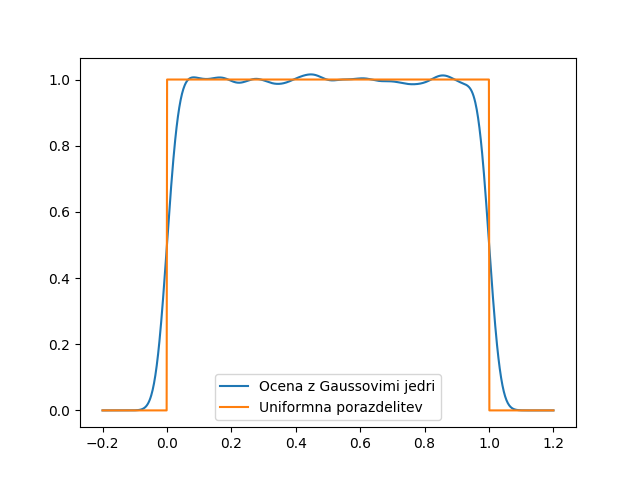
\includegraphics[width=0.45\textwidth]{gaussVSuniform.png}
    \caption{Vidi se, da ocena z Gaussovimi jedri preseže nosilec uniformne porazdelitve.}
\end{figure}
\pagebreak
Predstavili smo dva načina predstavitve podatkov. Obe načina predstavitve imata svoje prednosti in slabosti. Predstavitev s histogrami je zelo kompaktna, poleg tega pa histogram nikoli ne bo segal ven iz nosilca porazdelitve, saj je omejen s podatkovno množico. Pri ocenjevanju gostote verjetnosti z jedri se pa lahko zelo dobro približamo porazdelitvi, ki jo podatki predstavljajo, s čimer ne bomo izgubili nobene pomembne lastnosti podatkovne množice. Tvegamo pa, da lahko pademo ven iz nosilca.

Za naključen set podatkov, o katerem ne vemo nič, je težko reči, kateri način predstavitve je boljši. Vemo pa, da je za porazdelitve, ki imajo neskončne nosilce $(-\infty, \infty)$ in so gladke, veliko boljša predstavitev z oceno z Gaussovimi jedri. Pri porazdelitvah z omejenimi nosilci pa ta možnost odpade, tako da smo primorani operirati s histogrami.

Za konec tega poglavja pa predstavimo način, kako lahko optimalno število stolpcev iščemo z uporabo divergence. Kot primer vzemimo kar Kullback-Leibler divergenco $D_{KL}$.
\pagebreak

\subsection{Kullback-Leibler metoda za optimalno število stolpcev}

Naj bo $X = \{x_1, x_2, \ldots, x_n\}$ množica podatkov. Z oceno gostote verjetnosti množice $X$ z Gaussovim jedrom dobimo približek gostote verjetnosti $p$ množice $X$. Ta približek bomo primerjali s histogramom $h_n$ z n-stolpci s pomočjo Kullback-Leibler divergence po formuli:
\begin{equation}
    D_{KL}(p\|h_n) = \int_{\Omega}p(x)\cdot\log\Big(\frac{p(x)}{h_n(x)}\Big)\quad dx.
\end{equation}
Naredimo iteracijo po številu stolpcev $i = 1, \ldots, m$ za nek $m \in \mathbb{N}$. V vsaki iteraciji izračunajmo $D_{KL}(p\|h_i)$. Tisti $i$, pri katerem izraz doseže minimum, bomo vzeli za optimalno število stolpcev histograma množice $X$.

\begin{opomba}
    Zaradi zahtevnosti numeričnega računanja Kullback-Leibler divergenco v vsaki iteraciji raje računamo kot:
    \begin{equation}\label{KL-variate}
        D_{KL}(p\|h_i) = \int_\Omega p(x) \cdot ln(p(x)) dx - \int_\Omega p(x) \cdot ln(h_i(x)) dx.
    \end{equation}
    Na ta način lahko prvi člen izračunamo izven zanke, kar nam po izračunih privarčuje nekaj časa. Vemo pa tudi, da bo \eqref{KL-variate} minimalna natanko tedaj, ko bo $- \int_\Omega p(x) \cdot ln(h_i(x)) dx$.
\end{opomba}
\pagebreak
Poglejmo si, kakšne rezultate daje ta metoda v primerjavi z ostalimi.
\begin{figure}[!h]
    \centering
    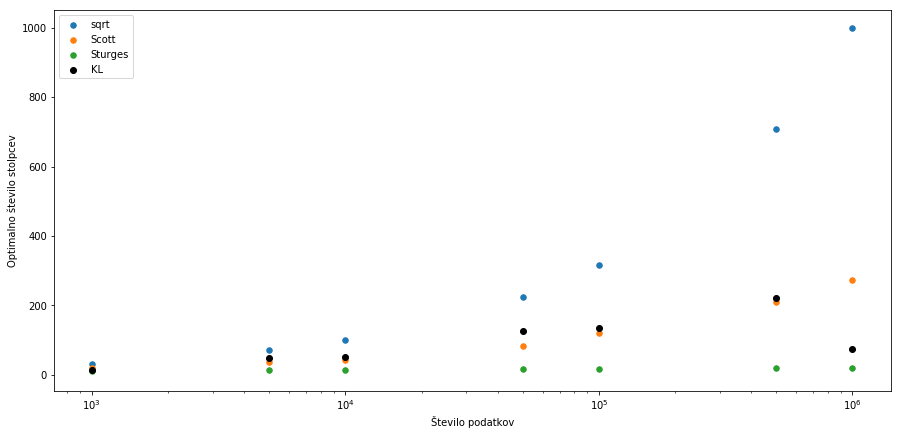
\includegraphics[width=\textwidth]{klVSostali}
    \caption{Primerjava med optimalnim številom stolpcev glede na korensko metodo in metodami Scott, Sturges in Kullback-Leibler. Os s številom podatkov je v logaritemski skali.}
\end{figure}

Zaradi preglednosti smo metodi Freedman-Diaconis in Rice izpustili. Iz slike je razvidno, da Kullback-Leibler metoda daje optimalna števila stolpcev podobna tistim, ki jih dajo ostale metode. Je pa izračun optimalnega števila stolpcev po Kullback-Leibler metodi zelo počasen, ko je število podatkov veliko. Prav tako pa procesa ne moremo optimizirati, saj funkcija $f(n) = D_{KL}(p\|h_n)$ ni konveksna, kar bi nam omogočilo iskanje minimuma, torej moramo direktno $m$-krat izračunati vrednost Kullback-Leibler divergence, kar pa je zaradi integriranja časovno zamudno.
